- Template matching - brukes sum of absolute differences SAD?

%Thus, the sonar image contains incomplete object information, and only contains partial object can only describe the object partially, can't be used to infer the object class unambiguously.


%
%Information is lost in the 
%
%Inferring the object class from the sonar image ambiguous, the sonar image ambiguous,  sonar image an ambiguous and suboptimal source to infer the object class from.

% This makes the sonar image represent the object ambiguously, and makes the class estimation unreliable.\todo{Not happy with this sentence}



%
%Object information is partially lost in the process, 
%
%Inferring object class from incomplete information.
%
%Since object information is lost in the process, 

%
%Thus, the sonar image ambiguously represent the object class Thus, the object class 
%
%
%Object ambiguously represented by the sonar image, and can't be inferred from it reliably.
%
%Sonar image represent the object ambiguously, making inference of 
%Inferring the object class from the sonar image is difficult, because it 
%
%Information is lost making the sonar image ambiguous, and inferring the object class hard.
%

%As a result the sonar image provide an ambiguous representation of the object.

%Information lost
%Sonar image ambiguous
%Inferring object class hard. 

% ambiguouslyInformation is lost in the process, preventing the object class can not be inferred unambiguously from the sonar image  The sonar image ambiguously describes the object class, and object class Inferring the object class from the sonar Information is partially lost in the process, making the sonar image an ambiguous representation of the object.\todo{bloated?}

%Inferring the object class from the sonar image

%Object information is irrevocably lost in the process, thus can no be inferred reliably from and  The resulting image e process is irreversible; No amount of guesswork To interpret and extract the needed information from these The image sought after may not be there, or take a form inconcievable for humans.

% Ideal parameters are unique and intrinsic---such type, shape, and size---, and independent of extrinsic features such as alignment, burial depth, degeneration level, or view angle.



 

%The challenge is to find unique and intrinsic object properties, such as type, shape and size, independent of extrinsic properties such as alignment, burial depth, degeneration level or view angle. 

%  comparable to optical cameras, but are harder to interpret; Acoustic effects such as layover, multiple scattering, diffraction, dispersion and penetration distort the image, making it an ambiguous representation of the object.

% Instead of trying to To bypass the intricacies of identifying a 3D object from an ambiguous 2D image, 

% Say how the templates come into existence first

% Instead of inferring object class from image, make a guess and compare simulation.

%Template matching bypass the problem of inferring the object class from the image, by guessing which object it is, 

%1. 3D model
%2. Acoustic simulation
%3. 
%
%An alternative approach consists of computing image templates for each object and orientation that may be 

% An alternative, called template matching, compares...
% Template matching differs by comparing the object...


%
%Numerous templates are required for each object, since every degree of freedom needed to describe it adds a dimension to the template solution space\todo{simplify}. 
%
%
%
%Feature for every degree of freedom - unmanageable 

% exponentially with every degree of freedom needed to represent the objects, adds number of templates needed to represent an object well grows exponentially with its number of degrees of freedom\todo{some way to simplify here?}.



% assuming similar sampling granularity of each parameter. 


%Template matching bypass the feature extraction by comparing the detected object with a set of simulated object templates, and assign it the class of the template with the best fit.\todo{reword somehow}  

%Template matching targets the ambiguity by instead starts with 3D models of relevant objects and orientations, simulates acoustic image templates for each, correlates them with detections\todo{vague} in the actual image, and estimates the class to be that of the template yielding the highest score.\todo{long, heavy, vague}   

%Template matching instead starts with 3D models acoustical image templates of probable objects and orientations, correlates them with detections\todo{vague} in the actual image, and estimates the class to be that of the template yielding the highest score.\todo{too heavy, vague} 

%Template matching instead starts with 3D models acoustical image templates of probable objects and orientations, correlates them with detections\todo{vague} in the actual image, and estimates the class to be that of the template yielding the highest score.\todo{too heavy, vague} 

%assigns records the scores. After iteration through all object classes and parameter configurations, the each detection is 

%roduce a template simulate how it would appears in a sonar image, and search the actual sonar image for similarities.  

%the deterministic acoustical effects distortions to produce an image template, and see if this resembles anything in the sonar image. This is called template matching.


%Template matching offers an alternative approach: Here an isolated image segment is compared to a set of template images covering the relevant object classes and orientations, and assigned to the class of the template with the best fit. Since the templates are computed from 3D models, this reduces the issue of image ambiguity. 

%However, it is challenging to find a static set of templates covering all suitable configurations of object and seafloor. Another issue is that the size of pre-computed library of templates grows exponentially with the number of parameters needed, assuming similar sampling granularity of each parameter. This limits its use to only a few parameters being coarsely sampled, ultimately yielding inaccurate results~\cite{Midelfart2010}.


% We avoid the problems of conventional template matching by computing the templates on-the-fly as part of the classification process, thereby not needing a precomputed set of templates at all. 
%  that avoids this problem by running sufficiently fast to create templates adapted to the actual scene as part of the classification process.
% Classification process


% Adaptive template matching:
% - To extract key features off the image

% Simulation of the templates:
% - To avoid static library of templates.
% - Less memory, better performance.


% To improve the reliability and efficiency, we propose two 
% reliability and efficient

%- AUV
%- ATR - feature extraction
%- ATR - template matching

%reduce feature solution space 


%\begin{itemize}
%\item Unified notation based on Gade.
%\item Sonar implementation.
%\end{itemize}

%Orthographic (projective) projection - parallel projection with the rays being perpendicular to the image plane.

%Simulating images of an active 100\,kHz SAS system share many traits to simulating optical images. Setting up the 3 dimensional scene is common to both, with the need to load various object models and setting up their interdependencies. Highlighting a region in the scene with acoustic energy can be modeled with a directional light source of equal beam width. Reflection models of light can be used too, since at 100\,kHz the acoustic waves mainly bounce off objects at their surface instead of penetrating them, and diffraction plays only a minor role. Finally, the resolution of modern SAS systems extend into the centimeter range in either direction. Combined these similarities can make it hard for an untrained eye to differentiate between a SAS and optical image.
%
%The big difference lies in what data is collected. A camera image represent a two-dimensional projection of a region of the scene onto an image plane. A sonar image, on the other hand, represent data from one fixed spatial dimension and range. 
%
%is that while an optical image is a projection plane purely in space, nsional space, the active sonar image is a projection of along-track an active sonar is a ranged sensor. With a phased array it captures data  It captures data 
%The main difference is the data format. While optical image represent the projection of all visible points in the camera view onto a projection plane, a sonar image captures data 
%
%
% in both along-track and cross-track, does not penetrate into the object  behave like that of light at 100\,kHz, with little penetration and  is high enough for waves not to penetrate into objects and Modeling reflections follow predominantly the same pattern, how sound reflect off various surfaces is dominantly similar to that of light,   with and comparable resolution. To make sure no Only letting the parts of the scene that is visible from the sconar The parts of the scene that is out of view Similar to an optical camera, an active sonar mainly receives echoes from the parts of the scene that is visible from the sonar. 
%
%In addition, SAS systems have high resolution making images look almost like optical ones. 
%
%sees the part of the scene that the A camera captures a represent a view-port on which that captures  The same way a camera only captures the part of the scene visible a part of the image with occluded parts being invisible, does Only the parts of the scene visible from from the camera and sonar pixels visible from the sonar will 
%
%
% is a sonar image is in many ways similar to those 
%Creating a 2D view of an arbitrary complex 3D scene is a non-trivial matter.  This is why we decided to use the core OpenGL pipeline to do this for us. OpenGL is a popular, well-matured and multi-platform application programming interface (API) for rendering 2D and 3D vector graphics. It relieves us from the intricacies of projecting vertices, faces and textures defined in a 3D space onto a suitable 2D image plane. This section explains how we set up OpenGL for this task, and then proceeds to describe how we post process the OpenGL images with OpenCL to form the final sonar image.
%
%\begin{itemize}
%\item Load arbitrary complex models
%\item Simulate sonar with OpenGL
%\item Speed considerations
%\end{itemize}
%
%Models are not ROCCAN (???)




% Euler angles
%    3 values
%    If few degrees of freedom, store only the ones needed
%    Gimbal lock

% Rotation matrices:
%    Allow transformation composition (sequence of multiplications)
%    9 values (for 3 degrees of freedom)
%    Easy to do e.g. strafing
%    Normalization necessary, but simulator recreates the matrices from scratch for each frame.
%    No Gimbal lock
%    Can include scaling, shear, reflection and translation (if 4x4)
%    4x4 matrices can also handle projective geometry.
%    Easy to work with and understand with a bit of linear algebra
%    Affine transformations. Nice analytical properties. Convenient.

% Axis-angle
%    Easy to interpolate angles
%    Hard to interpolate axes

% Quaternions
%%    Allow transformation composition (sequence of multiplications)
%    Specifies rotation through an axis and cos 0/2
%    4 values
%    Any two quaternions can be smoothly interpolated (blending) (just find the average)
%    If framerate drops below sampling rate (lag), then easy interpolation between two arbitrary frames is key.
%    No Gimbal lock
%    Faster (reference needed)
%    Easy to normalize / better numerical properties
%    Usually go-to solution for e.g. animations or games

% Rotors
%    Quaternions (4D complex numbers), thought of as 3D multivectors.

% More questions:
% - How to illustrate similar axes, e.g. system A shares first two basis vectors, but not last?

% Generally:
%    Semantics that prevent errors and force heightened awareness
%    Linting rules can be written to avoid errors

% Problems P V M
%    Where to put what? M or V?
%    How to relate physical quantities?
%    How to deal with a number of reference frames?
%    Too focused on editing individual axes / elements.
%    "If it doesn't work, flip some signs until it does"
%    Time-sink!

% T_AB
%    Every frame / coordinate system is has its own matrix. No need to think about where to put what. 
%    Decomposition is implicitly given.
%    Combines rotations, (scales,) and translations in one go. Higher abstraction to simplify design - hides the intricate details.
%    Hardly any trigonometric functions needed
%    Homogeneous coordinates - common formulation for both ordinary vectors and position vectors
%    Syntax relate allowed frames. Can't by mistake relate two incompatible systems without the notation revealing it.
% - Max/min syntax? Iŷẑ
% - xyz-coordinate of - say - I? Ix, Iy, Iz? Or, x_I, y_I, z_I?
% - L for linear 3x3 transforms?
%   
% - Need to standardize sets. I set of _I? How to denote size of dimensions?
% - Parallel, perpendicular? p||AB?
% - How to write out subscripts? 
% - Camelback in code for writing out letters? E.g. p_SonarClip_Sonar?
% - p_OI_xy, not working


% Blender internal is a biased rasterization engine, which means that it works by calculating which objects are visible to the camera and not by simulating the behavior of light.

%Models with rigid bodies - affine transformations preserve collinear properties.

% Future:
%   Cycles perform ray-tracing. Does this makes sense?

% Notation strategy
%   Avoid decomposed metrics if possible
%   Avoid working with individual axes is possible
%   Avoid use of Euler angles if possible
%   Keep notation as simple as possible without it being ambiguous
%   Linear ops change superscripts, translations change subscripts. Transformations change both.

% Quaternions: More computationally efficient, better numerical properties and simplifies interpolations.

% Homogeneous coordinates:
%   3x3: Linear operations such as rotations, scaling, shear, reflections
%   4x4: Include the 3x3, but also translation and perspective projection


%Vector based 
%aided with elegant, rigid and uniform notation system, based on points and reference frames.
%care is taken to define all needed points and reference frames, we 

% Huge scene, many object - ATR needed.

%Coordinates - unnecessarily details
%Frames and transforms, better abstraction level. Less errors.
%Not clear what coordinates in transformation mean. 
%
%
%Computer graphics 
%
%A common pitfall in computer graphics is to define geometries in terms of coordinates. 


%One of the most challenging aspects of computer graphics is dealing with geometries. We often need 3D models with different coordinate systems, where the vertices can represent either facets or quads, and their order and normals affect visibility (culling) and lighting. When smaller objects constitute bigger ones, they need geometrical interdependencies, applied such that the constituent's intrinsic properties remain intact and edible. Several cameras may be placed in the scene, but acting on these lead to an opposite effect in the scene; a camera moving right corresponds to the scene moving left. Finally, one need to decide how points in the scene are projected onto the image plane, keeping track of depth scaling, coordinate normalization and clipping. For games and animation timing also play a key role, with synchronization and interpolation challenges related to displaying the image on a screen. Yet, we have not touched advanced topics such as modeling realistic mechanics, materials, particles, or lighting---all requiring a strict grip on the scene's geometry.\todo{Too verbose}
%
%{\color{blue}Cherie: Bit wordy here as well... The point I just need to make is that computer graphics has complex geometrical dependencies, and to deal with these best one should work on a level of abstraction that doesn't involve dealing with coordinates whenever possible.}
%
%Traditional computer graphics literature express these geometrical relationships in terms of a model, view and perspective matrix---$\mat{M}$, $\mat{V}$ and $\mat{P}$, respectively. $\mat{M}$ is unique to each 3D model, and describes its placement in the scene. $\mat{V}$ represents the camera or observer, and describes how the scene moves when viewed differently. Finally, $\mat{P}$ describes how points visible to the camera projects onto a viewing plane\todo{A bit of overlap here with former paragraph. Perhaps drop this paragraph}. This is conceptually a good starting point, but provides no aid in defining the aforementioned complex effects.\todo{Too vague}


%The scene we seek to simulate 
%The scene we seek to simulate is 
%
%The first order of business is to define the 
%The simulator was designed with a certain set of functional requirements in mind: Sonar with monostatic Monostatic sonar, 
%The scene shown in \Fig{IV_simulator_coordinate_system} fulfills these criteria.
%
%Monostatic sonar
%Arbitrary position
%
%
%
%The 
%Scenes 
%We seek the Transitions involving a rotation and a translation are called affine transformations, and are of key interest because they preserve rigid bodies.




%Rotations fall into the category of linear transforms. If the model size was incorrect we seek another linear transform: scaling. To generalize  Often we also want other candidates from this category, such as scaling, reflection or shearing. 

%To change the decomposition we multiply with some linear transform $\mat{L}\colon\mathbb{R}^3\!\to\!\mathbb{R}^3$. Gade restricts these to rotation matrices, which preserve lengths and cross-products---a prerequisite for rigid body transformations~\cite{Murray1994}. Computer graphics deal with this extensively, but not exclusively; Linear effects such as scaling, shear and reflection are sometimes needed.

%Since linear transforms generally are non-commutative, the notation system specifies the proper sequence of multiplication in the subscripts of $\mat{L}_{ED}$; Vectors or other linear transformation matrices decomposed in $\uvec{D}$ go to the right, while those in $\uvec{E}$ go to the left.\todo{$\mat{R}_{ED} = \mat{R}_{DE}^T$ (usually)} Note that representing the vector differently does not change it; its direction and magnitude remains unchanged.

% SE(3) Lie group with the axioms:
% - If A,B   in SE(3), then AB in SE(3)   (set is closed under binary operation)
% - If A,B,C in SE(3)m then (AB)C = A(BC) (binary operation is associative)
% - For every A in SE(3) there exist a I in SE(3) such that AI=A
% - For every A in SE(3) there is an inverse A^-1 in SE(3) such that AA^-1 = I
% SE(3) is a continuous group, i.e. the binary operation is continuous => if differentiable
% The inverse of any element in SE(3) is a continuous function of that element
% A group with a differentiable manifold is called a Lie group.



%- All terms must have same decomposition (superscript).
%- Closest points should be identical and cancel (in subscript).
%- Resulting subscript Decomposition same, and unchanged.
%



%The simulator architecture and notation system are described Section~\ref{IV_methods}. Simulation and classification results  Results from  template simulations and classification Section~\ref{IV_results}  Finally, we present classification performance using 
%
%, and supply a Python snippet to demonstrate it.Section???
%In Section . 
%
%\todo{Introduce sections}

% Mathematical formulation/notation: Simulation, Robotics

%We will explore the classification performance of these two techniques, but otherwise 
%In this study we focus on describing the simulator, but compare classification results from both methods to that of standard template matching. 
% but provide some details on adaptive template matching for completeness where needed. 






%We will show that:
%%
%\begin{itemize}
%\item Adaptive template matching improves classification performance compared to its conventional peer,
%\item Improved classification performance by feeding simulator with parameters derived off SAS image,
%\item Further improved classification by performing a fine-search within a narrow search space around the SAS derived parameters. GPU makes this more powerful.
%\end{itemize}

% This is achieved with the aid of the massive computing power in graphics processing units (GPUs) and optimized software libraries for scene rendering. The simulator loads a 3D model of the seafloor and object class into OpenGL and positions the camera at the sonar location. The scene is highlighted using a light tube that extends to infinity along the AUV's axis of probagation. We assume rough, isotropic surfaces reflecting sound energy equally in all directions. This can be modeled with a Lambertian scattering model~\cite{Blake1993,Bell1995}, where the intensity of the backscattered sound solely depends on the incidence angle of the transmitted signal onto the model surface. The OpenGL rendering produces an optical 2D intensity image and depth map that reveals the distance from each pixel to the propagation axis. For maximum flexibility this data is finally combined with OpenCL to produce the image templates.

%as part of the classification process. This is achieved with the aid of the massive computing power in graphics processing units (GPUs) and optimized software libraries for scene rendering.

%The simulator loads a 3D model of the seafloor and an object class model into OpenGL, where emitted sound waves are modeled with a cylindrical light source placed at the sonar transmit location. 

%We assume rough, isotropic surfaces reflecting sound energy equally in all directions. This can be modeled with a Lambertian scattering model~\cite{Blake1993,Bell1995}, where the intensity of the backscattered sound solely depends on the incidence angle of the transmitted signal onto the model surface. When rendering OpenGL is set up to produce an optical 2D intensity image and depth map that reveals the distance from each pixel to the propagation axis. For maximum flexibility this data is finally combined with OpenCL to produce the image templates.


%For lack of a better name, the simulator will be referred to as "FFISim" throughout this article.

%



%

%
%Although this does the job, we combine this into a single operation by using homogeneous coordinates. 
%
%Seek a higher abstraction level to unify all these operations.

%Active transformation moves the points. Wish to transform this group of points but retain the relation between them. Need affine transform, consist of a linear transform and a translation.
%%
%\begin{align}
%\vec{p}_{MV} &= \vec{R}\,\vec{p}_{MV} + \vec{t},\label{eq_position_vector}
%\end{align}
%%
%$\vec{R}$ can be defined in various ways, e.g. with Euler-Rodrigues in Euclidean $\mathbb{R}^3$ space which rotates about an axis $\hat{r}$ by angle $\theta$. 

%
%$V_t$ relates to $\ubar{I}$ as $\udot{V}$ relates to $\ubar{M}$.

%$\big(\vec{R}_{IM},\vec{p}_{IM}\big)$ uniquely specifies how $\ubar{I}$ relates to $\bar{M}$ and contains $2N$ degrees of freedom. Unique and geometrically clear, but tuples are inconvenient to work with. Odd because vector not moving, only representation. Decomposed notation describe this unambiguously.
%
%Free:
%Geometrically unambiguous
%
%Decomposed:
%Matrices instead of tuples
%Clear on passive/active
%Better suited for frames
%
% - Transformation explicit on being active or passive
% - Logical validitiy
% 
%Suppose we wish to move $\udot{V}$ and the rest of the rigid body. Need translation and rotation. 
%
% 1. Define points & frames
% 2. Translate/rotate position vectors
% 3. Increase abstraction: The R3 transform / homogeneous coordinates
% 

%Change a point: Add position vector / translation.
%Change a set of vectors: Rotate each - axis-angle, quaternions, matrices.

%
%Rotations:  All pros cons. Matrices nice formal properties, but ambiguous. How to specify representation? 
%
%

%Projections (non-linear) with linear algebra -> homogeneous coordinates
%Vectors: Linear space - space of vectors - foundation of traditional linear algebra 3D vectors
%Points: Affine space - space of points - foundation of computer graphics
%
%Deal with points, not vectors. Points can only be combined through affine combinations, not linear ones(?)
%
% ADT coordinate-free, conceptually clear, inefficient(?)

%Suppose we wish to represent our geometric elements in $\mathbb{R}^3$ Euclidean space, to support the notion of lengths, dot- and cross-product.

%A set of rules accompany the notation system to validate and describe operations; Subscripts can only be changed by translations, and superscripts by linear transformations. To start with the former, consider the following summation:

%Vector-vector operations like summation, dot- and cross-product, only makes sense when the vectors are decomposed in the same vector space---easily verified by the superscripts. The subscripts explain how the vector is altered: The intermediate (closest) frames cancel each other, leaving the start and end frame as subscript for the resulting vector. This mimics the regular rules of vector addition.

%\begin{align}\nonumber\\[.5\baselineskip]
%\dvec{p}_{\g{AC1}{AC}}^{\g{E1}{A}}
%= \mat{T}_{\g{A2}{A}\r{B1}{B}} \; \dvec{p}_{\r{B2}{B}\g{C1}{C}}^{\r{B2}{B}}\label{eq_transform}
%\\[.5\baselineskip]\nonumber
%\tikz[overlay,remember picture]{
%%   \coordinate(A) at  ($ .5*(E1)  + .5*(A2) $);
%  \path let \p1 = (E1), \p2 = ($.5*(E1)+.5*(A2)$) in coordinate (A) at (\x2,\y1);
%%  \path let \p1 = (E1), \p2 = ($.5*(AC1)+.25*(B2)+.25*(C1)$) in coordinate (AC) at (\x2,\y1);
%  \path let \p1 = (AC1), \p2 = ($.7*(AC1)+.15*(B2)+.15*(C1)$) in coordinate (AC) at (\x2,\y1);
%  \path let \p1 = (E1), \p2 = ($.5*(B1)+.5*(B2)$) in coordinate (B) at (\x2,\y1);
%  \path let \p1 = (E1), \p2 = ($.5*(E1)+.5*(B2)$) in coordinate (Sup) at (\x2,\y1);
%%  \coordinate(B) at  ($ .5*(B1)  + .5*(B2) $);
%  \coordinate(AB) at ($ .5*(AB1) + .5*(AB2) $);
% \node(Re)[above = 1.5\baselineskip of B, anchor=center]%
%   {\footnotesize\textrm{Closest frames identical and cancel}};
%    \draw[->](A2.north) to[out=90, in=0] ($ (A)+(0em,3.2ex) $) to[out=180,in=90] (E1.north);
%    \draw[->](B2.north) to[out=90, in=0] ($ (B)+(0em,3.2ex) $) to[out=180,in=90] (B1.north);
%%   \node(ABe)[below = 1.5\baselineskip of AB, anchor=center]%
%%     {\footnotesize\textrm{Unchanged}};
%%    \draw[->] (AB2.south) to[out=-90, in=0]($ (AB)+(0em,-3.2ex) $) to[out=180,in=-90] (AB1.south);
%    \draw[->](C1.south) to[out=-90, in=0]($(AC.south)-(0em,3.2ex)$) to[out=180,in=-90]($ (AC1.south)-(0,0ex)$);
%    \draw[->](A2.south) to[out=-90, in=0]($(AC.south)-(0em,3.2ex)$) to[out=180,in=-90]($ (AC1.south)-(0,0ex)$);
%%    \draw[->, in=-90, out=-90] (A2.south) to ($ (AC.south) - (0,0ex)$);
%}
%\end{align}
%
Note that for this operation to be valid the input vector must match the transformation matrix \emph{both} in decomposition (superscript) and closest frame in the subscript.



%$\mat{L}_{AB}$ and $\mat{S}_{AB}$$\mat{S}_{AB}$ are a rotation and scaling matrix that converts from frame $B$ to $A$,
% Affine
% - Preserve points, straight lines and planes.
% - Sets of parallel lines remain parallel.
% - Combination of a linear transform and a translation.
% 
% Projective space
% - 
%
%
%      Representation/decomp.       Subscript
%      Input          Output        Input            Output
% Add  Same           Unchanged     Closest cancel   Farthest remain
% Mul  Closest match  Left remain   Don't care       Unchanged
% T



\subsubsection{Model placement}

Combining the two aforementioned operations---a linear transformation (\ref{eq_vector_multiplication}) and a translation (\ref{eq_vector_addition})---result in an affine transformation. Like the These preserve points, straight lines and planes, and ensure collinearity (parallel lines remain parallel). This is important dealing with rigid objects either in the physical world or as here---virtually. We can produce a single affine transformation as follows$\in\mathrm{SE}(N)$\todo{Add some fireworks}\todo{Add a note on projective spaces?}:
%
\begin{align}\label{eq:T_definition}
\mat{T}_{AB}
= \left[\begin{array}{c c c | c}
& & &   \\
& \mat{L}_{AB}  & & \dvec{t}_{AB}^A \\
& & &  \\\hline
 0 &  0  &  0  &  w
\end{array}\right] 
\end{align}
%\begin{cases}
%\in \mathrm{SO}(3)  & \mathrm{if $w\in\{0,1\}$} \\
%\in \mathrm{Sim}(3) & \mathrm{otherwise.}
%\end{cases}
%= \mat{R}_{AB}\;\mat{S}_{AB}      = \dvec{p}_{AB}^A
where $\mat{L}_{AB}: \mathbb{R}^3 \to \mathbb{R}^3$ and $\dvec{t}_{AB}^A$ represent the linear map and translation from $\udot{B}$ to $\udot{A}$, respectively.




\subsubsection{General geometry}


%
%he transitions between them follow a unified pattern, and it becomes easier to think in terms of vectors instead of coordinates. This keeps even large systems manageable and removes a frequent source of error.
%
Every transformation follows the format defined in \eq{eq:T_definition}. For all linear maneuvers in the scene, their contents are summarized in Table \ref{tab_transformation_contents}:
%
\begin{table}[h]\normalsize\centering
\begin{tabular}{r c c r c c}
	\hline
	\rowcolor{tabBlue}                     & $\mat{T}_{XC}$      & T$_{CO}$                & $\mat{T}_{OS}$      & $\mat{T}_{SI}$      & $\mat{T}_{IM}$             \\ \hline
	$\mat{L}$ in (\ref{eq:T_definition})   & See (\ref{eq_L_XC})      & See (\ref{eq_cart2cyl}) & $\mat{R}_{OS}$      & $\mat{I}$           & $\mat{R}_{IM}\mat{S}_{IM}$ \\
	$\dvec{t}$  in (\ref{eq:T_definition}) & $\boldsymbol{0}$ & See (\ref{eq_cart2cyl}) & $\dvec{p}_{OS}^{O}$ & $\dvec{p}_{SI}^{S}$ & $\dvec{p}_{IM}^{I}$ \\
   & & & \multicolumn{3}{c}{World space} \\
   & & & \multicolumn{3}{c}{Affine} 
\end{tabular}%
\caption{Affine transformation contents}\label{tab_transformation_contents}
\end{table}
%
where
%
\begin{align}
\mat{R}_{IM} &= \mat{R}(\psi,\theta+\pi,\phi), \\
\mat{S}_{IM} &= \text{diag}(\dvec{s}_{IM}^I),
\intertext{and}
\mat{R}_{OS} &= \mat{R}(\uvec{I}_{\,z}^S, \dvec{p}_{SI}^{S}).
\end{align}
%
where $\mat{R}(\psi,\theta,\phi)$ are user specified roll, pitch and yaw,\todo{Update table for Euler-free angles}\todo{How to lose the arrow without this looking like a matrix? It's decomposed...} and $\uvec{I}_{\,z}^S = \mat{T}_{SI}\bmat{0,0,1}\T$.




%To get an idea of the geometries involved we refer to \Fig{IV_simulator_coordinate_system}. 

%Our models are stored in regular 3D model files. The simulator loads these into a tree of nodes, each representing a vertex in the model with corresponding facet and texture information. Then the vertices are placed into a virtual scene in OpenGL, and a camera set up to capture the part of the scene corresponding to the image. When OpenGL renders the image, it first computes which vertex contributes to which pixel in the image, then computes the intensity and color of the pixel based on the node's facet, texture and scattering model. In computer graphics terminology, the code that operates on vertices are called a vertex shader, and the code that operates on pixels are called a fragment shader.

%Before we describe the rendering pipeline in further detail, 

%In computer graphics 
%Contrary to many computer graphics applications, we 

%
%We represent the translation $\vec{p}_{IM}$ in $\uvec{I}$ as
%%
%\begin{align}
%\dvec{p}_{IM}^I&\in \mathbb{R}^3,
%\intertext{the rotation $\vec{R}_{IM}$ in $\uvec{I}$ as}
%\dvec{R}_{IM}&\in\mathrm{SO(3)} \colon \mathbb{R}^3 \to \mathbb{R}^3,
%\intertext{and combine these together into the displacement $\vec{T}_{IM}$ in $\uvec{I}$,}
%\dvec{T}_{IM}&\in\mathrm{Sim(3)} \colon \mathbb{R}^4 \to \mathbb{R}^4
%\end{align}
%
%



% %
%  Since $\dvec{p}_{MV}'^M$ only differs from $\dvec{p}_{MV}^M$ by the appended one. 
% This is an affine transformation, one that preserves  the They guarantee the preservation of rigid bodies. Because other linear operations are sometimes needed, such as scaling, reflection and shearing, we may generalize \eq{eq_rotation_translation} by swapping $\dvec{R}_{IM}$ with $\dvec{L}_{IM}$. 





% effektivt - høyere grad av abstrakthet
% serie av projeksjoner, uniform

%
%$(\psi,\theta,\phi) = (
%
%where the position vector $\dvec{p}_\textit{\tiny{}SI}^\textit{\tiny{}S}$ specifies translation to the image ($I$) center in sonar ($S$) coordinates and the linear transformation matrix $\mat{L}_\textit{\tiny{}SM}$ encodes scaling and rotation information. The transformation \eq{eq:M} is also affine as long as the bottom row is $(0,0,0,1)$.


%\begin{align}
%\M = \bmat{
%  &    &    &   \\
%  &    &    & \dvec{p}_\textrm{\tiny{}SI}^\textsc{\tiny{$S$}}$ \\
%  &   &    &   \\
%0  &  0  &  0  &  1 \\
%}
%\end{align}

%$\ubar{I} = (\udot{I},\uvec{I}) = (\udot{S}+o^\textit{S},\uvec{S}$.
%
%Where $\dvec{v}_{}^L = [x,y,z,w]\T$ denote vertex $v$ decomposed in reference frame $L$, with the homogeneous coordinates $L$, $v = \bmat{ x\,w & y\,w & z\,w }$ 
%
%%Sonar coordinate frame, denoted $\p^S$. Models denoted $\p^M$.
%
%
%
%
%The model matrix $\M_\mathrm{WM}$ is applied first to the object to convert it from its local "model" space to world space. It is defined as:
%
%\begin{align}
%\mat{R}_{IM} = \mat{R}_{IM} \mat{S}_{IM}
%\end{align}
%
%where $\boldsymbol{S}$, $\boldsymbol{R}$ and $\boldsymbol{T}$ are transformation matrices that sets the object's scale, rotation and translation, respectively. Combined these transforms map the object from its local coordinate system to the world's coordinate system. They are provided for reference in Appendix \ref{IV_transformation_matrices}.

%Next the object is mapped into world coordinates with the view matrix $\V$. This involves aligning the camera to precisely fit the image region. In our case the camera represents the phase center of the sonar, and it is placed in the world origin. The transformation then take the form of
%
%\begin{align}\label{eq:M}
%\mat{T}_{SI}
%= \left[\begin{array}{c c c | c}
%& & &   \\
%& \mat{R}_{SI}(0,0,0) & & \dvec{p}_{SI}^{S} \\
%& & &  \\\hline
% 0 &  0  &  0  &  1
%\end{array}\right]
%\end{align}
%%
%\begin{align}\label{eq:M}
%\mat{T}_{OS}
%= \left[\begin{array}{c c c | c}
%& & &   \\
%& \mat{R}_{OS}(\frac{\pi}{2}-\text{atan}\left(\frac{\dvec{p}_{SI,z}^{S}}{\dvec{p}_{SI,y}^{S}}\right),0,0) & & \dvec{p}_{OS}^{O} \\
%& & &  \\\hline
% 0 &  0  &  0  &  1
%\end{array}\right]
%\end{align}
%%
%where
%%
%\begin{align}
%\mat{L}_{SI} = \mat{R}_{SI} \mat{S}_{SI}
%\end{align}



%\begin{align}
%\V &= \mat{T}(\c^\mathrm{W}) \cdot \R_\text{x}(\phi_x, 0, 0) \nonumber\\
%&= 
%\bmat{
%1  &  0  &  0  &  c_\text{x} \\
%0  &  1  &  0  &  c_\text{y} \\
%0  &  0  &  1  &  c_\text{z} \\
%0  &  0  &  0  &  1 \\
%} \cdot
%\bmat{
%1  &  0           &  0           &  0 \\
%0  &  \cos\phi_x  &  -\sin\phi_x &  0 \\
%0  &  \sin\phi_x  &  \cos\phi_x  &  0 \\
%0  &  0           &  0           &  1 \\
%},
%\end{align}
%
%where $(x_\text{c}, y_\text{c}, z_\text{c})$ is the image center coordinates for along track, cross track, and depth, respectively, and $\phi_x$ is the elevation angle\todo{is this correct?} of the sonar. It is given as
%%
%\begin{align*}
%\phi_x &= \arctan\left(\frac{y_\text{mean}}{-z_\text{mean}}\right).
%\end{align*}\todo{use absolute sign?}


%
%\begin{align}
%\P = \left(\begin{matrix}
%\frac{2}{r-l}  &  0              &  0              &  -\frac{r+l}{r-l} \\
%0              &  \frac{2}{t-b}  &  0              &  -\frac{t+b}{t-b} \\
%0              &  0              &  \frac{-2}{f-n} &  -\frac{f+n}{f-n} \\
%0              &  0              &  0              &  1
%\end{matrix}\right)
%\end{align}
%%
%where $l,r,b$ and $t$ are the left, right, bottom and top boundaries of the projection plane, respectively, and where $n$ and $f$ is the near and far limits of the cube that encompass the scene. These parameters need to be adapted to provide a 2D image that matches the image size, which we specify in along track and cross track coordinates ($x,y$). This is straightforward for left and right since matches the $x$-axis
%% They define the window through which we observe our scene.
%\begin{align}
%l &= x_\text{min}  &  r &= x_\text{max}
%\end{align}
%%
%For the near and far limits one simply needs to make sure the scene will fit in it, say
%%
%\begin{align}
%n &= 0\;\text{m}   &  f &= 300\;\text{m}.
%\end{align}
%%
%The bottom and top boundaries can be inferred from \Fig{IV_camera_top_bottom}. First we define an origin vector that points to the center of the image
%%
%\begin{align}
%\vec o &= \left[\frac{x_\text{min}+x_\text{max}}{2}, \frac{y_\text{min}+y_\text{max}}{2}, \frac{z_\text{min}+z_\text{max}}{2} \right]\T,
%\end{align}
%%
%and the distance from the image origin to its $y$-boundaries is given as
%%
%\begin{align}
%\Delta y &= \frac{|y_\text{max} - y_\text{min}|}{2}.
%\end{align}
%%
%To find the nearest and farthest point in the image that will be part of the projected scene, $\alpha$ and $\beta$, we must consider the seafloor rotation angle around the $x$-axis, $\Phi_x$ 
%%
%\begin{align}
%\vec\alpha &= \vec 0 - \left[0, \Delta y, \Delta y \cdot \tan\Phi_\text{x} \right] \nn
%\vec\beta &= \vec 0 + \left[0, \Delta y, \Delta y \cdot \tan\Phi_\text{x} \right]
%\end{align}
%
%\begin{figure}[t]\centering%
%\includegraphics[drawing,width=\linewidth]{gfx/opengl_part.svg}%
%\caption{Setting camera top and bottom boundaries.}\label{IV_camera_top_bottom}%
%\end{figure}
%


%Map from $\mathbb{R}^{MxN} \rightarrow \mathbb{R}^{MxN}$




%\subsection{Template matching}
%
%1. Segmentation
%2. Parameter estimation
%   Available: Range, altitude, resolution => Input to both standard and adaptive. In standard the best fit out of a predefined template database is selected, then resampled to correct resolution.
%   Additional for adaptive, parameters that modify object model: Target aspect angle, seafloor slope, object length and height.
%
%   Target aspect angle computed with Radon Transform, seafloor under object modeled as plane with a slope estimated from bathymetric data, length estimated from longest part of highlight region, and height estimated from the shape of the shadow. The burial depth is n
%
%
%   
%3. 
%
%   Details: \cite{Midelfart2010}.
%
%Let $S(x,y)$ be the isolated part of the
%
%Matching the isolated image segment with the template take the form of
%
%\begin{align}
%c_{h,i} = \underset{x',y'}{\text{argmax}} \sum\limits_{\forall x}\sum\limits_{\forall y} \big| H(x,y) - T(x-x',y-y') \big|
%\end{align}
%
%\begin{align}
%c_i = \frac{c_{h,i} + c_{s,i}}{2}
%\end{align}
%
%And the final template used is the one with the greatest correlation coefficient
%
%\begin{align}
%\underset{T_i(x,y)}{\text{argmax}} C_i\sum\limits_{\forall x}\sum\limits_{\forall y}  S(x,y) T(x-x',y-y')
%\end{align}
%
%Then assign object to class $i$.
%
%
%To narrow down the search space of possible templates we derive some reliable statistics of the seafloor and object from the SAS image. While FFISim accepts an arbitrarily complex seabed, we find that modeling it as a plane wave with the right tilt works well. The object is more difficult. For instance, we estimate its length and height from the shape of its shadow, but this fails if the object is notably immersed into the seabed at one end. 
%
%After the a template is created we decompose it into its highlight and shadow component, and compute a correlation score between these and the corresponding areas in the SAS image. Then the two scores are summed and normalized to form the final correlation score of the template.
%
%We tag the template matchers as either semi- or fully adaptive. The former refers to using the best matching SIGMAS+ generated template out of a precomputed set of templates, while the latter refers to the proposed method of using FFISim to generate templates on the-the-fly. \todo{Should be more precise. How many templates? Parameter span? How finely were the parameters sampled?} 

% It is also possible to compute the sonar image using the OpenGL ``blend'' feature.




% lists every frame configuration s the configuration of every frame transition, along with constraints and representation.

% Thus, $\mathcal{C}_M\in\mathbb{R}^N\times{}S^2\times{}S^1$, where $\times$ denotes the cartesian product of sets. 

% The configuration space $\mathcal{C}_{IM}=(\vec{p}_{IM},\vec{R}_{IM})\in \mathbb{R}^N\times{}S^2\times{}S^1$.
%
%The image frame $\ubar{I}$ can be defined relative to $\ubar{M}$, by relating their positions by a position vector $\vec{p}_{IM}$ going from $\udot{I}$ to $\udot{M}$,
%%
%\begin{align}
%\vec{p}_{IM} \triangleq \udot{M} - \udot{I},\label{eq_position_vector}
%\end{align}
%%
%and their orientations by a rotation operator $\vec{R}_{IM}$,
%%
%\begin{align}
%\vec{R}_{IM} \colon \uvec{M} &\to \uvec{I}\nn
%\vec{m} &\mapsto \vec{i}.\label{eq_rotation_dyadic}
%\end{align}
%


%
%   $\vec{p}_{IM}$, for instance, specifies the image frame's position $\udot{I}$ relative to $\udot{M}$.
%
%It can be  defined relative to $\ubar{M}$, by relating their positions by a position vector $\vec{p}_{IM}$ going from $\udot{I}$ to $\udot{M}$,
%%
%\begin{align}
%\vec{p}_{IM} \triangleq \udot{M} - \udot{I},\label{eq_position_vector}
%\end{align}
%%
%and their orientations by a rotation operator $\vec{R}_{IM}$,
%%
%\begin{align}
%\vec{R}_{IM} \colon \uvec{M} &\to \uvec{I}, \quad
%\vec{m} \mapsto \vec{i}.\label{eq_rotation_dyadic}
%\end{align}
%
%If $\vec{p}_{IM}$ defined we can connect Its position is defined by $\vec{p}_{IM}$
%Frame positions are related similarly. $\vec{p}_{IM}$, for instance, specifies the image frame's position $\udot{I}$ relative to $\udot{M}$.
% The position vectors share the same $N$ linear degrees of freedom as the positions on which they rely, and must be adressed through parametrization and constraints.
%When all the scene's frames connect either directly or indirectly through position vectors, any non-existing connection between two points to be made with the head-to-tail axiom,
%


%According to the Chasles-Mozzi theorem, any rigid body displacement can be composed from a rotation and a translation. 
%
% To preserve model rigidity, all the model's vertex-vectors can only be together by a single affine operation; First a rotation (or more generally, a linear transformation) for changing its orientation, followed by a translation for changing its position.
%
% $N$ of which defines position with a topology of $\mathbb{E}^3S^2S^1$ ($N=3) or $\mathbb{E}^2S^1$ $N$ of which defines position and the rest orientation. The topology In an $N=2$ dimensions, Its topology 
%
%The translation has $N$ linear degrees of freedom, , and .
%The rotation can either specify orientation, rotate a point, or change representation.
%
%The model is rigid, so the ratios of lengths between its points must be constant. This is ensured when the model's vertices
%
%
%
%The model $\vec{p}_{MV}$ transformed by a combination of a linear shift $\vec{t}$   and rotation $\vec{R}$
%%
%\begin{align}
%\vec{p}_{MV'} &= \vec{R}\vec{p}_{MV} + \vec{t}\label{eq_position_vector_translated}
%\end{align}
%
%or rotated with a rotation operator $\vec{R}$
%%
%\begin{align}
%\vec{p}_{MV'} &= \vec{R}\vec{p}_{MV}\label{eq_position_vector_rotated}
%\end{align}
%
%
%Given a model vertex $\vec{p}_{MV}$, we can use \eq{eq_position_vector} to translate it
%is applied to a  we can use \eq{eq_position_vector} relative to the model, we define a position vector $\vec{p}_{MV}\in\mathbb{V}$ going from $\udot{M}$ to $\udot{V}$,
%


%The configuration of $\mathcal{M}$ can be specified by a vector $\dvec{p}\in\mathbb{R}$ describing $\udot{M}$ with respect to $\udot{I}$, and a rotation matrix, $\mat{R}_{IM}
%$, whose columns describe the relative orientation of axes of $\ubar{M}$ with respect to those of $\ubar{I}$.

%\begin{tabular}{l l l}
% model body       & $\mathcal{M}$ & $\ubar{M}$  \\
% workspace/world  & $\mathcal{W}$ & $\ubar{W}$
%\end{tabular}

%
%Many geometrical concepts can be described without coordinate systems. Doing so promotes geometrical reasoning conceptually The fundamental properties of a point or a vector do not depend on A point or line, they exist This promotes conceptual clarity when modeling the physical reality.   
%
%Most computer graphics literature describe geometrical concepts using coordinates and matrices. Although readily implementable, a bit of geometrical clarity is lost in the process.  the  in a computer, . Stacked into matrices, the However, many geometrical concepts are independent of the choice of coordinate systems, a
%
% The solutions are readily implementable, but The trouble is that Although this provide readily implementable Although However,  coordinates introduce ambiguities many geometrical concepts can be described in a coordinate-free manner. s. We emphasize some of these by first this by first To emphasize this, wecan be do not rely on these are better described using coordinate-free notation. Although While this is certainly needed to implement 

%Consider the scene in \Fig{IV_simulator_coordinate_system}, where an object model resides on the seafloor.

% Euclidean
% Orthonormal  ($\hat{m}_i\in\mathbb{V}$ being the $i$-th orthonormal basis vector)

%{
%\setlength\tabcolsep{0pt}%\def\arraystretch{1.5}
%\begin{align*}
%	\t{M} \quad Model            \\
%	\t{I} \quad Image           \\
%	\t{S} \quad Sonar                                         \\
%	\t{O} \quad Orthogonal view                               \\
%	\t{C} \quad Cylindric view                                \\
%	\t{X} \quad Clip             
%    \tikz[overlay,remember picture]{}
%\end{align*}

%\begin{filecontents*}{table.tex}
%\begin{tabular}{l*{3}{c}}
%& A & B & C \\
%\hline
%1 & blah & blah & blah \\
%2 & blah & blah & blah \\
%3 & blah & blah & blah \\
%\hline
%\end{tabular}
%\end{filecontents*}
%\begin{tikzpicture}
%\matrix[ampersand replacement=\&] {
%\node (tables1) [shape=rectangle,draw] {
%\begin{tabular}{l l}
%\end{tabular}
%};
%};
%\end{tikzpicture}
%\node(table) {
%	\t{M} & Model            \\
%	\t{I} & Image           \\
%	\t{S} & Sonar                                         \\
%	\t{O} & Orthogonal view                               \\
%	\t{C} & Cylindric view                                \\
%	\t{X} & Clip };             
%    \tikz[overlay,remember picture]{}


            





%}
%
%\tikz[overlay,remember picture]{
%  % Set up some general bounding box markers
%  \coordinate(CC) at ($ .5*(CL)  + .5*(CR) $);
%  \coordinate(TC) at ($    (CC)  + (0em,1.3\baselineskip) $);
%  \coordinate(BC) at ($    (CC)  - (0em,1.3\baselineskip) $);
%  % Compute means
%  \coordinate(AB) at ($ .5*(A1)  + .5*(B1) $);
%  \coordinate(BC1) at ($ .5*(B2)  + .5*(C1) $);
%  % Compute arrow via points
%  \path let \p1 = ($.5*(AC) +.5*(A1)$),   \p2 = (BC) in coordinate (A)      at (\x1,\y2);
%  \path let \p1 = ($.5*(AB) +.5*(BC1)$),  \p2 = (BC) in coordinate (AB_BC)  at (\x1,\y2);
%  % Draw arrows and text
%  \node(De)[above = 2\baselineskip of CC, anchor=center]%
%    {\footnotesize\textrm{Same frame}};
%    \draw[<-, in=-90, out=90] (D1.north) to ($ (De.south) + (0,1ex)$);
%    \draw[<-, in=-90, out=90] (D2.north) to ($ (De.south) + (0,1ex)$);
%    \draw[<-, in=-90, out=90] (D3.north) to ($ (De.south) + (0,1ex)$);
%  \node(ACe)[below = 2\baselineskip of CC, anchor=center]%
%    {\footnotesize\textrm{Change of vector}};
%    \draw[->] (C1.south) to[out=-90, in=0] (AB_BC) to[out=180, in=0] (A) to[out=180, in=-90](AC.south);
%    \draw[-] (A1.south) to[out=-90, in=0] ($ (A)+(0em,0ex) $);
%    }

%It relies on reference frames and transitions between these. 

%To showcase the advantage of using our notation system, observe from \Fig{IV_simulator_coordinate_system} which reference frames we decomposed the virtual scene into: A 3D model $\ubar{M}$, image region $\ubar{I}$, sonar local body $\ubar{S}$, and an orthogonal and cylindric viewing plane, $\ubar{O}$ and $\ubar{C}$, respectively. The sequence of affine transforms that a vertex $\udot{V}$% $\dvec{v}^\textit{\tiny{}M}$
%for model $M$ undergo is given as\todo{Condense sequence to improve speed}:
%
%
%It takes as input a "rigid" model of the object and seafloor, and transforms them in several steps to produce the image template.
%
%
%orthogonal to the slant-range; mmodel of a object and seafloor as viewed from the sonar, and OpenCL converts this information into an image template. 
%

%
%
%Referring same points from different locations. frames
%
% The models are rigid, meaning
%
% ---contains is a fairly complex 
%
%Complex scenes containing rigid bodies---such as the one in \Fig{IV_simulator_coordinate_system} that underpins our simulator---
%
%can often be described elegantly in terms of reference frames.
%
%Given as input an object and seafloor model undergo a set of transformations to produce the image template, described as a transition from one frame to another. In the spatial domain these are usually affine, the kind that involves a rotation and a translation, because they preserve the model structures. 

%Affine transformations can be described in an clear, organized and robust manner with a 


%%In computer graphics the geometrical transitions are often expressed as a single transformation We extend Gade's notation to also 
%However, we extend it to  however, extend it 

%uniformly


%Thinking in terms of these matrices are fine in the beginning, but for more complex scenes it is not clear when to use which. The issues arise when trying to deal with complex scenes with the aforementioned effects.

% is easy to understand, but where does fine initially, but but the real challenge lies in defining these matrices---say if you try to model a physical system with multiple reference frames, physical constraints and some non-linear features\todo{Awkward. Not convincing.}.
 
%
% 
%Prefer vectors, 
%Notation leads the way

%Occlusion 
%Culling
%Normals
%Handedness

%About half the time developing the simulator was spent dealing with the (slightly simplified) geometries illustrated in \Fig{IV_simulator_coordinate_system}; It was far too easy to get lost when compounding transforms, thinking in terms of coordinates rater than vectors, and when dealing with various corner-cases.\todo{Too verbal} However, this was later rectified by adopting and extending the stringent and unified notation system developed by Gade~\cite{Gade2018}. We present a subset of his (simplified) notation here, before extending it to homogeneous coordinates and projective spaces---which are a better fit to computer graphics.



%Reference frames, transitions between them. Leads to uniform process.

% Coordinate based approach
% - Heavy use of matrices to describe geometric operations
% - Multiplication with [2,0;0,1] might mean: Changed coordinate system but same geometry, same coordinate system but changed geometry, a map from one domain to another, or it may have no geometric interpretation at all.
% Without keeping track of coordinate system/spaces, it's easy and common to make mistakes. In particular, to perform geometrically meaningless operations such as combining points or vectors from different spaces.

% Coordinate-free
% - Address problem of ambiguity and validity by sticking to geometric reasoning.
% - Geometric objects implementation pixar reference. Ensures that only valid geometrical operations are performed.

% Affine spaces
% - More general foundation for Euclidean space. Points have the single attribute position, while free vectors have a direction and magnitude.
% - Subtraction axiom:
%   v = P-Q     for every P,Q     (no "points at infinity")
%   P-Q = v     for every Q,v     (no "holes" in the space)
% - Head-to-tail-axiom
%   (P-Q)+(Q-R) = P-R
%
% Claims:
% Q-Q = 0 (vector)
% R-Q = -(Q-R)
% v+(Q-R) = (v+Q)-R
% P = Q + (P-Q)
% (Q+v)-(R+w) = (Q-R)-(v-w)

% Frames
% - Most familiar (physical) way to coordinatize affine space (one other being simplexes)
% - The "configuration" of affine space, just like bases in vector space

% Homogeneous coordinates.
% + Convenient
% - 4 instead of 3 dimensions
%
% logical spaces

%Geometrical objects: Points. Vectors act on points. Rotation matrices act on vectors.

%The transformation of a rigid body in Euclidean space is uniquely defined by a translation and a rotation. 

%Rigid objects. Cloud of points with fixed distances between them. Transform that preserve this property comprised of translation of origins, plus a rotation of bases. Abstract away these and coordinate-specific details. Only talk about transforms.


%Notation categories: With and without coordinates. First, coordinate-free. Pure geometrical reasoning, geometrical elements and associated operations, higher abstraction, conceptually clear, close relation to physical reality. Then, represent geometrical objects with coordinates. Ambiguities and numerical side effects easier to handle with a firm grasp of geometric reasoning.



%- Template quality FFISim/SIGMAS+, similar. Same size/shape.
%- Adaptive technique for highlight, tie for shadows. Same seen in segmentation result.
%- Speed -> FFISim


%Note how the adaptive technique excels at reproducing accurate highlights, but that this does not necessarily translate into accurate shadows. 

%In terms of template quality both SIGMAS+ and FFISim produce similar results. 

%\Fig{IV_fig_image_simulation} contrasts the segmentation result of the templates with that of the SAS image---in terms of highlight, shadow and background regions. As expected the adaptive technique generally produce better matching templates, but with a surprising caveat: Improved highlight scores did not necessarily translate to better shadow scores. 


%Out of the objects in the scene we selected a 2.6\;m long cylinder that was partly buried in the sea sediments (Fig. \ref{IV_data_cylinder}). The length, immersion depth and aspect angle of this cylinder were estimated from the SAS image using our  adaptive template matching approach~\cite{Midelfart2010}. 

%Then these parameters were used by the simulator to create an adaptive template (Fig. \ref{IV_sim_cylinder}), which is an almost perfect match of the cylinder. We also created standard templates for a regular template matching approach. In this case, we assumed that the cylinder mine had a generic length of 2\;m (like a MP80 or a Murena mine) and was proud on the seafloor. Moreover, templates were created for every 10$^\text{th}$ degree of the aspect angle. We believe these assumptions to be typical for a template library for cylinder mines. 

%Note how the adaptive template obtained a much closer fit to image than the standard template. This was also reflected in the correlation scores (which were created with the method described in \cite{Midelfart2010}) that were 0.613 for the standard template and 0.813 for the adaptive template. Hence, the standard approach was less likely to classify the cylinder in the image correctly as the standard templates were not created specifically for the target.

%The main difference lies in how they integrate into the classification process: While SIGMAS+ generate one template for each invocation, FFISim can iterate through a space of parameters on the GPU before returning control to the CPU. This speeds up the template matching dramatically, allowing it to assess thousands of templates per second instead of, say, one. 

% FFISim provide templates that better match the true object orientation in this figure, but  

% Different background level. Adaptive technique excels for less normal objects/geometries.
%Overlap - Provide quantification measure. 



 
%- Stm stimulated with length matching test cylinder. Perfect score against this.
%- Atm - not given to improve score. Shadow and highlight both need to match, and overfitting could lead to reduced performance.
%
%
%
%
%Good statistics drawn from the image -> adaptive better. Poor statistics -> hit and miss.
%
%
%1. Comparison with standard template library (ROC enough?)
%   ROC: Adaptive better at FPR<0.2 in all cases.
%2. Comparison with SIGMAS+
%   Fairly similar images, performance is similar. 
%   Used to create the standard template library.
%3. Comparison with search space
%   ROC: Additional search always better FPR<0.2.
%   Explain search criterion.



%SAS images - look good. Random pick objects. Lengths derived from image.


%
%1. Adaptive better? Compare with standard. Doing this in ROC
%2. Improved classification? ROCs
%3. Further improvement by doing fine-search? ROC
%
%
%An issue the adaptive technique must deal with when estimating object length 
%
%As the ROC curves indicate, the adaptive template matching techniques both  ROC curves demonstrate the 
%
%The majority of the objects in the Jesus Bay are cylinder shaped. A SAS image of three such objects are displayed in \Fig{IV_fig_image_sonar}
%
%
%
%


% \begin{figure*}[!tbp]\centering%
% \subfloat[SAS images of 2 cylinders and a torpedo.]{%
% \includegraphics[width=0.5\linewidth]{gfx/fig_images_sonar_simulation.pdf}%
% \label{IV_fig_sonar_simulation}}%
% \subfloat[Cylinder simulation with parameters estimated from SAS image: Length 2.6\;m, burial depth 0.263\;m, aspect angle 105$^\circ$.]{
% \includegraphics[drawing,width=0.5\linewidth]{gfx/sim_cylinder_submerged_adaptive.svg}%
% \label{IV_sim_cylinder}}%
% \caption{A SAS image of a cylinder and a template simulation adapted to it.}
% \end{figure*}
% 
% 
% \begin{figure*}[!tbp]\centering%
% \subfloat[SAS image of a cylinder with 2.6\;m length and 0.53\;m radius.]{%
% 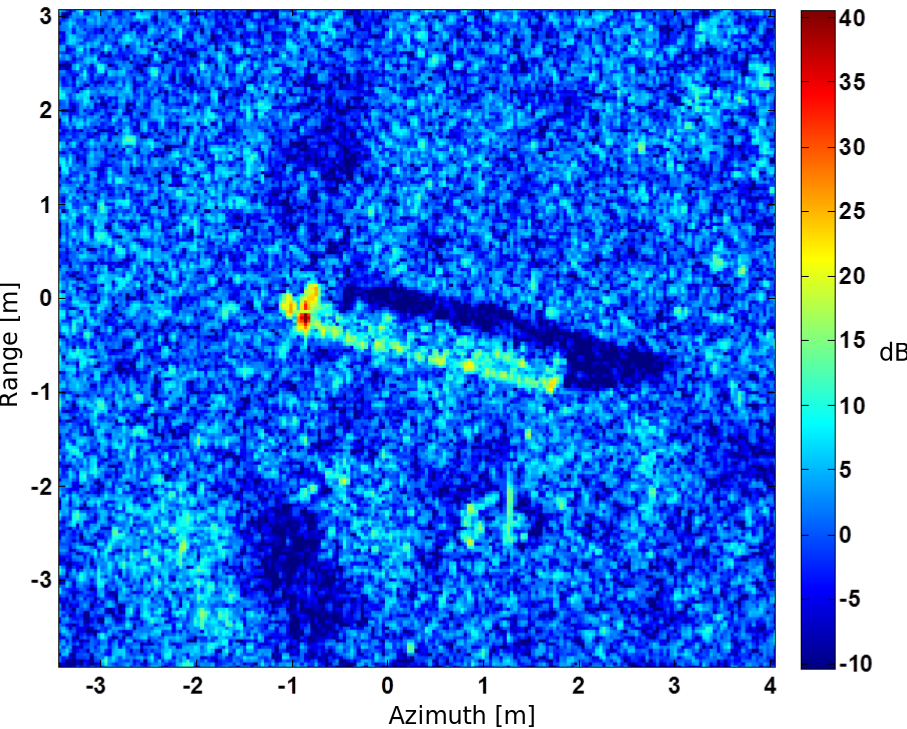
\includegraphics[drawing,width=0.5\linewidth]{gfx/data_cylinder_submerged.svg}%
% \label{IV_data_cylinder}}%
% \subfloat[Cylinder simulation with parameters estimated from SAS image: Length 2.6\;m, burial depth 0.263\;m, aspect angle 105$^\circ$.]{
% \includegraphics[drawing,width=0.5\linewidth]{gfx/sim_cylinder_submerged_adaptive.svg}%
% \label{IV_sim_cylinder}}%
% \caption{A SAS image of a cylinder and a template simulation adapted to it.}
% \end{figure*}


% \newcommand\cdesc[2]{#2}


% Whenever conventional computer graphics processing can be used to 
% GPUs are designed to provide the best possible graphics processing performance, and there large ecosystem of tools and libraries  available 
% Using a GPU to drive a simulator is advantageous since
% 
% 
% Creating a GPU-based simulator is attractive since computer is an attractive solution as there are a  graphics traits. For one over a CPU-based standard simulator is two-fold: 



%
%
%
%\begin{itemize}
%\item GPUs low power. Good for integration in AUVs.
%\item Good accuracy even with a real-time constraint in e.g. a AUV.
%\item Improved inertial navigation?
%\item Aid in understanding the key parts of the SAS image and in discovering potential flaws in the SAS image. Anomalies can be flagged to make SAS more robust?
%\end{itemize}
